\documentclass{article}
\usepackage{stackengine}
%\usepackage[utf8]{inputenc}
\usepackage[T1]{fontenc}
\usepackage{amsmath}
\usepackage{amsfonts}
\usepackage{graphicx}
\usepackage{pbsi}
\usepackage{lmodern}
%\usepackage{tgbonum}
\usepackage[a4paper]{geometry}
\usepackage{pdflscape}
\usepackage[dvipsnames, svgnames]{xcolor}
\usepackage[pages=some]{background}
\usepackage{tikz}
\usetikzlibrary{math} 
\usetikzlibrary{automata,positioning}
\usetikzlibrary[decorations.text]
\usetikzlibrary{arrows.meta} % LATEX and plain TEX when using Tik Z
%\usetikzlibrary[automata]
\usetikzlibrary{calc}

\newcommand\BackImage[2][scale=1]{%
\BgThispage
\backgroundsetup{
scale=1,
angle=0,
opacity=1,  %% adjust
contents={\includegraphics[width=\paperwidth,height=\paperheight]{#2}}
%contents={\includegraphics[#1]{#2}}
}
}

\newcommand*{\vertchar}[2][0pt]{%
  \tikz[
    inner sep=1pt,
    shorten >=-.15ex,
    shorten <=-.15ex,
    line cap=round,
    baseline=(c.base),
  ]\draw
    (0,0) node (c) {#2}
    ($(c.north)+(#1,0)$) -- ($(c.north)+(#1,0)$);%
}


\makeatletter
\newcommand{\dotr}[1]{%
  \mathpalette\@dotr{#1}%
}

\newcommand*{\@dotr}[2]{%
  % #1: math style (\displaystyle, ..., \scriptscriptstyle)
  % #2: argument of \dotr
  \sbox0{$\m@th#1#2$}%
  \usebox{0}%
  % simulating a superscript
  %\raisebox{\dimexpr\ht0-\height}{$\m@th#1\addvbuffer[-1ex 0.9ex]{.}}%
  \raisebox{3.5pt}{$\m@th#1\@smallbullet#1\bullet$}%
  \kern\scriptspace
}
\newcommand*{\@smallbullet}[2]{%
  \scalebox{.3}{$\m@th#1#2$}%
}
\makeatother
    
\newcommand*{\siin}[1]{\stackinset{c}{}{b}{5.5pt}{\small\ttfamily\char'15}{#1}}
\newcommand*{\nn}{\textsuperscript{n}}

\newcommand*{\pehin}[1]{\stackinset{c}{}{b}{5.5pt}{\small\ttfamily\char'15}{#1}}
\newcommand*{\dtr}{\raisebox{3.5pt}{$\scalebox{.3}{$\bullet$}$}}
\newcommand*{\dtrh}{\raisebox{5pt}{$\scalebox{.3}{$\bullet$}$}}



\begin{document}


\hspace*{-15mm}
\resizebox{18cm}{!} {
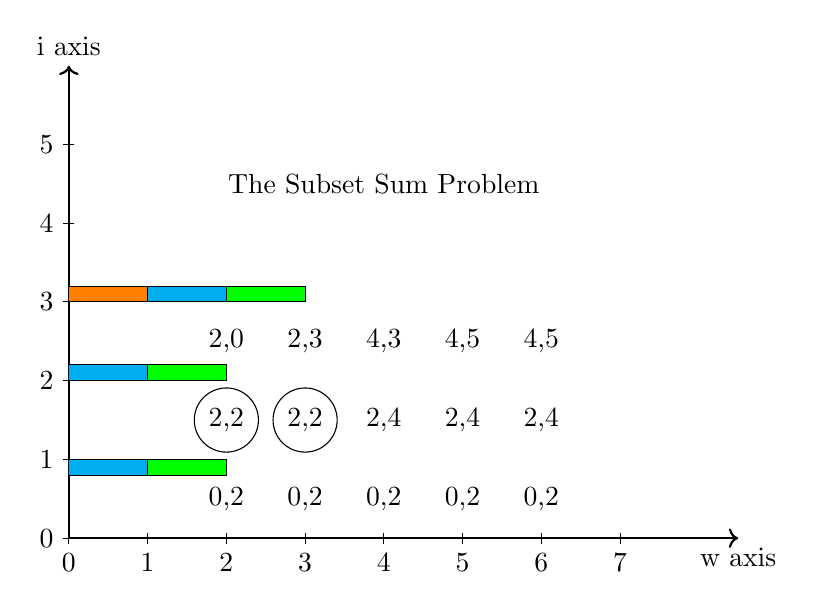
\begin{tikzpicture} 

\foreach \x in {0,...,7}
   \draw (\x cm,2pt) -- (\x cm,-2pt) node[anchor=north] {$\x$};
\foreach \y in {0,...,5 }
    \draw (2pt,\y cm) -- (-2pt,\y cm) node[anchor=east] {$\y$};
\draw[thick,->] (0,0) -- (8.5,0) node [anchor= north]{w axis};
\draw[thick,->] (0,0) -- (0,6) node [anchor= south] {i axis};

\filldraw [fill=orange] (0,3) rectangle (1,3.2);
\filldraw [fill=cyan] (1,3) rectangle (2,3.2);
\filldraw [fill=green] (2,3) rectangle (3,3.2);
\filldraw [fill=cyan] (0,2) rectangle (1,2.2);
\filldraw [fill=green] (1,2) rectangle (2,2.2);
\filldraw [fill=cyan] (0,0.8) rectangle (1,1);
\filldraw [fill=green] (1,0.8) rectangle (2,1);

\foreach \x in {2,...,6} 
  \node at (\x, 0.5) {0,2};

\path (2, 1.5) node[circle, inner sep=.1cm, draw] {2,2}
(3, 1.5) node[circle, inner sep=.1cm, draw] {2,2};

\foreach \x in {4,...,6} 
  \node at (\x, 1.5) {2,4};

\path (2, 2.5) node {2,0}
(3, 2.5) node {2,3}
(4, 2.5) node {4,3}
(5, 2.5) node {4,5}
(6, 2.5) node {4,5};

\draw (4,4.5) node {The Subset Sum Problem};

\end{tikzpicture}
}

\vspace*{10mm} 
\hspace*{3mm}
{\LARGE Subset Sum Problem size W=6, items \(w_1\)=2,\(w_2\)=2, \(w_3\)=3}

\end{document}